\documentclass{beamer}

\usepackage{graphicx}
\usepackage[sfdefault,light]{FiraSans}
%\usefonttheme{serif} 
\usepackage[british]{datetime2}
\usetheme{default}
\setbeamertemplate{navigation symbols}{} % No navigation symbols
\setbeamercolor{alerted text}{fg=blue!80!green!159!}
\setbeamercolor{frame title}{fg=blue!80!green!159!}
\setbeamercolor{title}{fg=blue!80!green!159!}
\setbeamercolor{subtitle}{fg=blue!80!green!159!}

\makeatletter
\setbeamertemplate{footline}
{
  \leavevmode%
  \hbox{%
  \begin{beamercolorbox}[wd=.15\paperwidth,ht=2.25ex,dp=1ex,center]{institute in head/foot}%
    \usebeamerfont{title in head/foot}%
    \raisebox{-0.15cm}{
\includegraphics[width=1cm]{logo_ntnu_u-slagord.pdf}}
  \end{beamercolorbox}%
  \begin{beamercolorbox}[wd=.6\paperwidth,ht=2.25ex,dp=1ex,center]{institute in head/foot}%
    \usebeamerfont{title in head/foot}%
    \insertsection
  \end{beamercolorbox}%
  \begin{beamercolorbox}[wd=.15\paperwidth,ht=2.25ex,dp=1ex,center]{institute in head/foot}%
    \usebeamerfont{title in head/foot}%
    \insertshortdate
  \end{beamercolorbox}%
  \begin{beamercolorbox}[wd=.1\paperwidth,ht=2.25ex,dp=1ex,right]{institute in head/foot}%
    \usebeamerfont{title in head/foot} 
    \insertframenumber{} / \inserttotalframenumber\hspace*{2ex} 
  \end{beamercolorbox}}%
}
\makeatother

%----------------------------------------------------------------------------------------
%	TITLE PAGE
%----------------------------------------------------------------------------------------

\title{POL2012: Theories and Models in Political Economy}
\subtitle{Classical Political Economy}
% \date{\today}
\date{}
\author{Marius Swane Wishman}
\institute{Department of Sociology and Political Science}

\begin{document}

\begin{frame}[plain]
\titlepage % Print the title page as the first slide
\centering % Comment out if second logo

\includegraphics[width=5cm]{logo_ntnu_u-slagord.pdf}
%\hspace{0.5cm} 
\includegraphics[width=5cm]{logo_ntnu_u-slagord.pdf} % Second logo
\end{frame}


\section{Historical context} % Sections can be created in order to organize your presentation into discrete blocks, all sections and subsections are automatically printed in the table of contents as an overview of the talk
%------------------------------------------------


\begin{frame}{Historical Context - The Emergence of Capitalism}
\begin{itemize}[<+- | alert@+>]
    \item Expansion of trade
    \item Improvements in agriculture
    \item Population growth
    \item Revolutions
\end{itemize}
\end{frame}

\begin{frame}{Historical Context - The Emergence of Capitalism}
    \begin{figure}
        \centering
        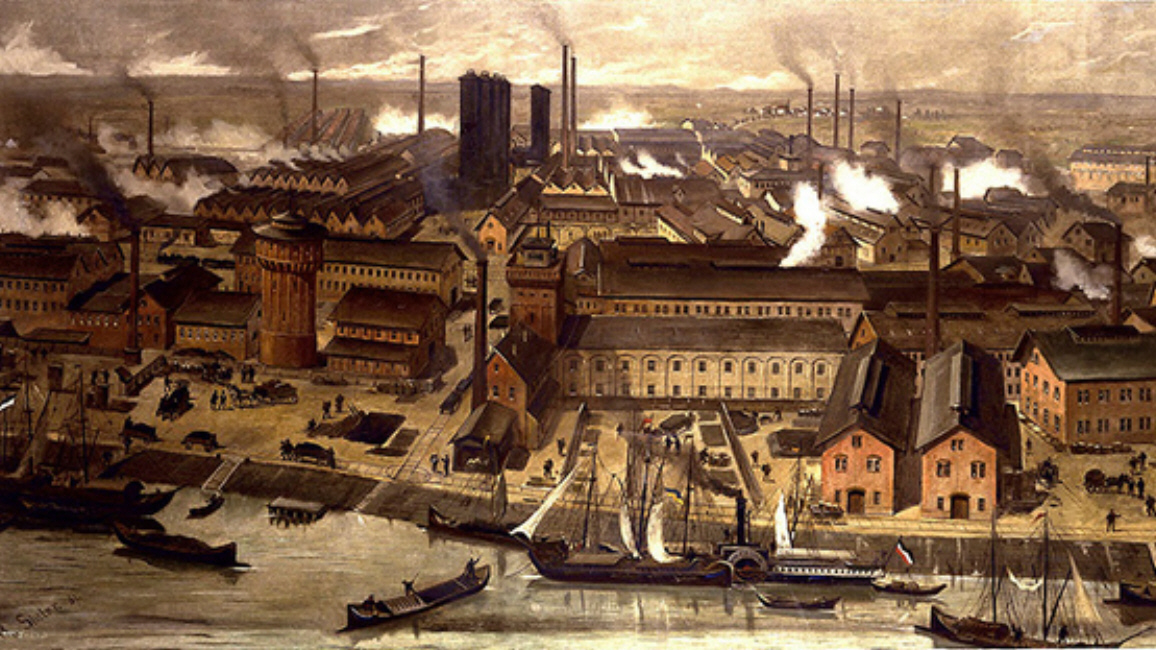
\includegraphics[width=\textwidth]{../img/industry.JPG}
        \caption{Industrial Revolution}
    \end{figure}
\end{frame}{}

\section{Adam Smith (1723-90)}
\setbeamertemplate{background}{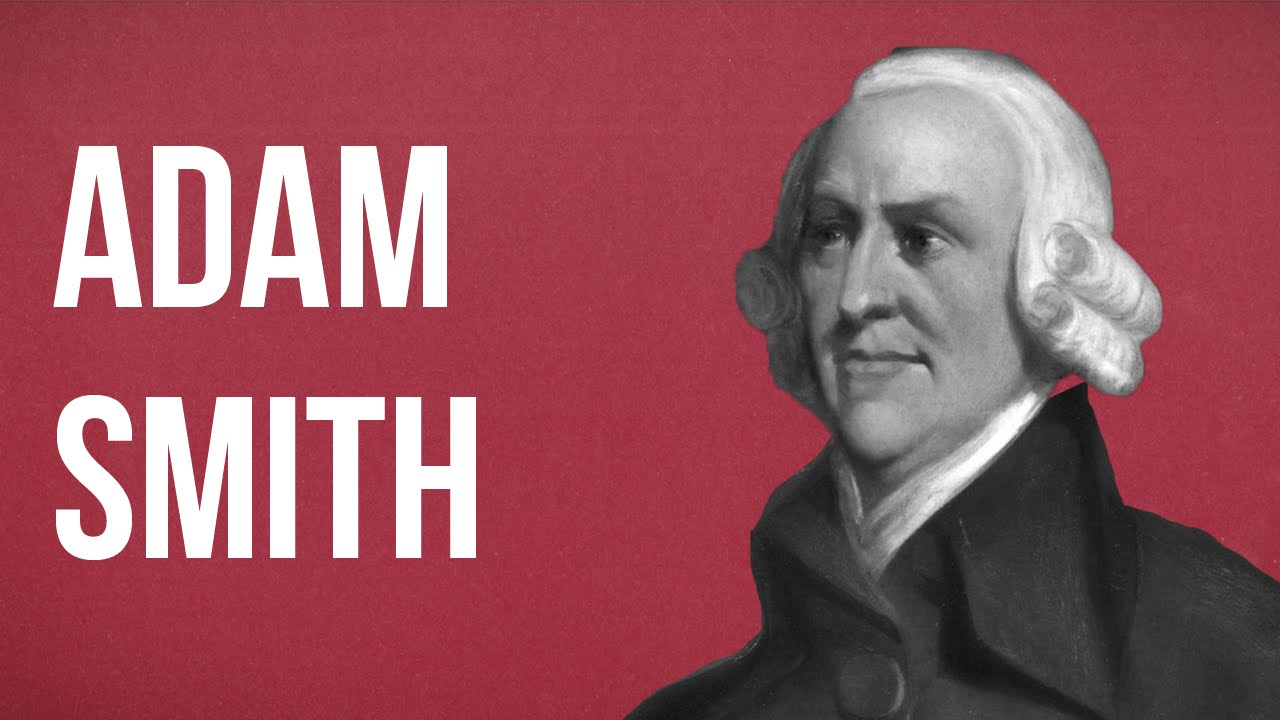
\includegraphics[width=\paperwidth, height=\textheight]{../img/smith.jpg}}

\begin{frame}{}

\end{frame}{}

\setbeamertemplate{background}

\begin{frame}{Adam Smith (1723-90)}
    \begin{figure}
        \centering
        
\includegraphics[width=0.5\textwidth, height=0.5\textheight]{../img/invisiblehand2.jpg}
        \caption{The Invisible Hand}
    \end{figure}
\end{frame}{}

\begin{frame}{Adam Smith (1723-90)}
    \begin{itemize}[<+- | alert@+>]
    \item Changing values 
    \item Mercantilism
    \item "Just prices"
    \item Competition and market prices $\neq$ laissez-faire
    \item Division of labor
    \end{itemize}
\end{frame}{}

\begin{frame}{Adam Smith (1723-90)}
What is the theory?
\end{frame}

\section{David Ricardo 1772-1823}
\begin{frame}{David Ricardo 1772-1823}
      \begin{figure}
        \centering
        \includegraphics[width=0.9\textwidth, height=0.9\textheight]{../img/banana.jpg}
    \end{figure}  
\end{frame}{}

\begin{frame}{David Ricardo 1772-1823}
    \begin{itemize}[<+- | alert@+>]
    \item Absolute advantages
    \item Comparative advantages
    \end{itemize}
\end{frame}{}

\begin{frame}{Comparative Advantage}
    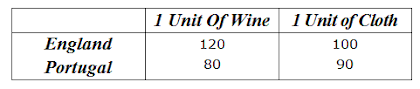
\includegraphics[width=5cm]{../img/David-Ricardo-England-Portugal-Wine-Cloth-Principle-of-Comparative-Advantage.png}
    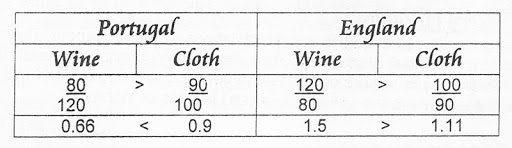
\includegraphics[width=6cm]{../img/Cost-Ratios-of-Producing-Wine-Cloth-Portugal-England.jpg}
\end{frame}{}

\begin{frame}{Comparative Advantage}
    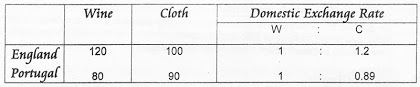
\includegraphics[width=7cm]{../img/Comparative-Cost-Benefits-Both-Participants.jpg}
\end{frame}{}

\begin{frame}{David Ricardo 1772-1823}
    \begin{itemize}[<+- | alert@+>]
    \item Class as a product of source of income
    \item Interaction between landowners, capital and labor
    \end{itemize}
\end{frame}{}

\section{Thomas Malthus (1766-1823)}
\begin{frame}{Thomas Malthus (1766-1823)}
      \begin{figure}
        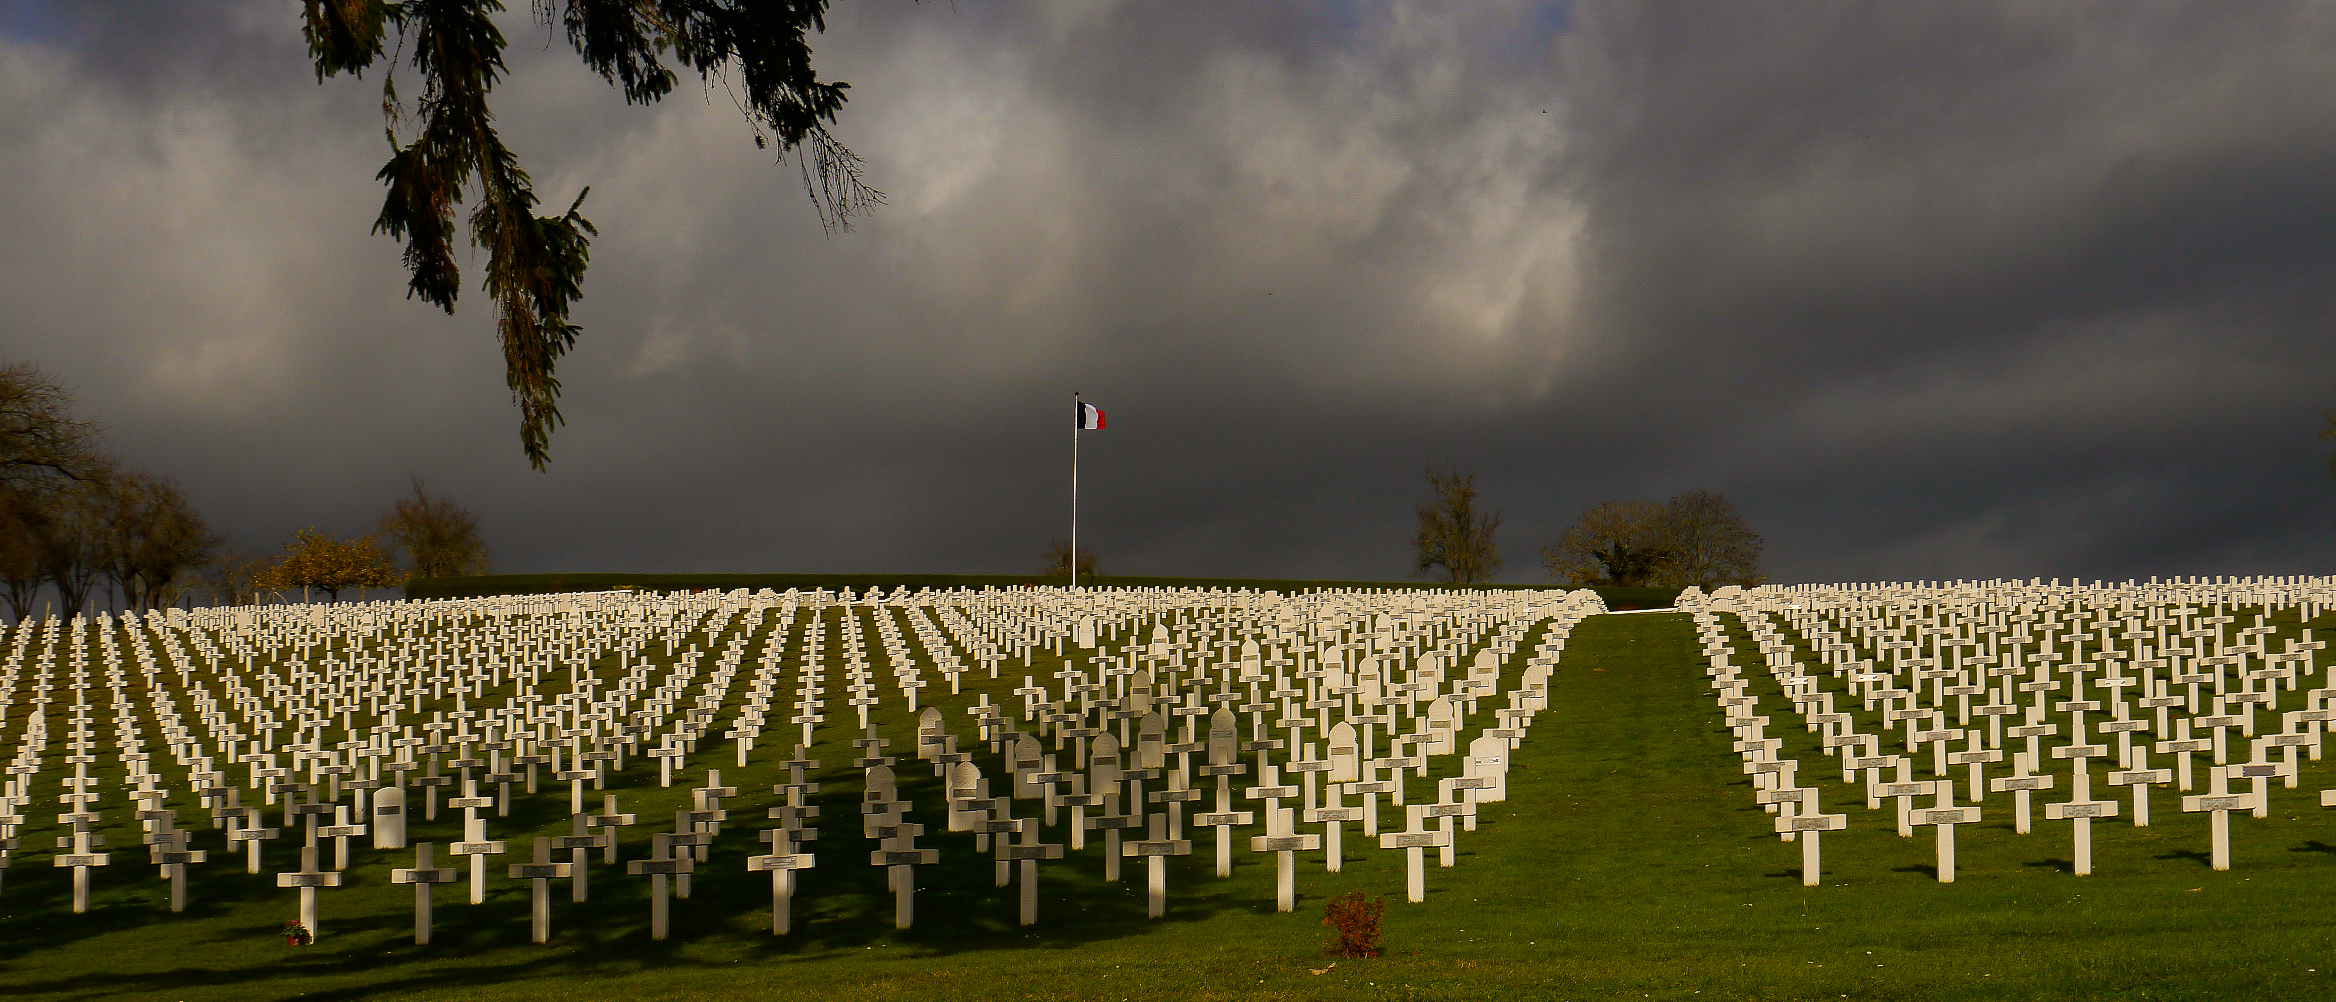
\includegraphics[width=\textwidth, keepaspectratio]{../img/malthus.jpg}
    \end{figure}  
\end{frame}{}

\section{Jean-Babtiste Say (1767-1832)}

\begin{frame}{Jean-Babtiste Say (1767-1832)}
\begin{figure}[htpb]
	\centering
	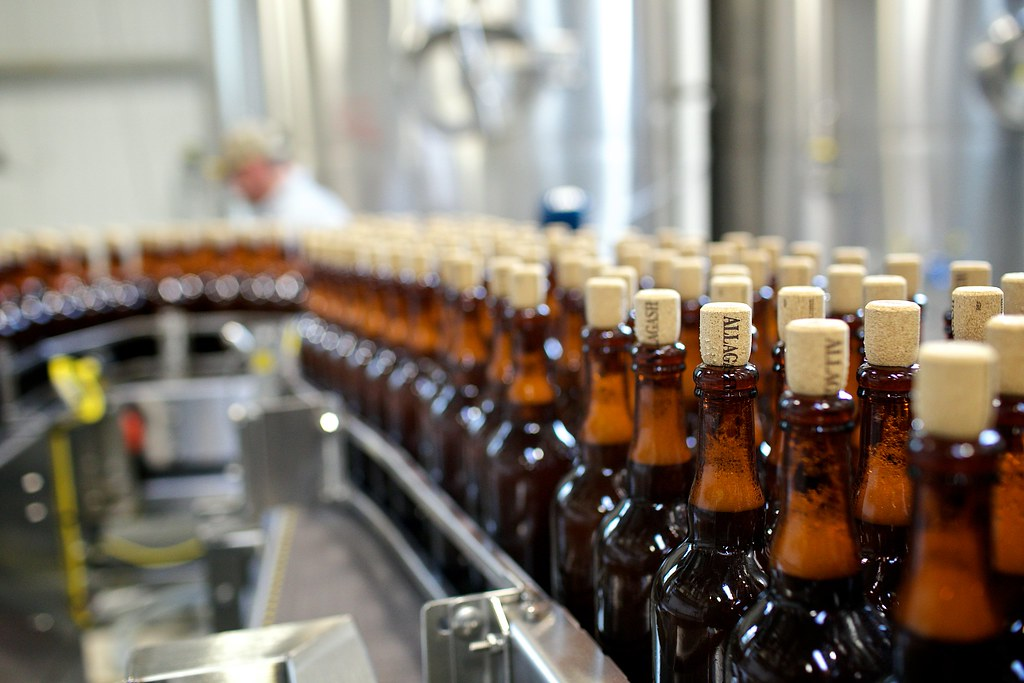
\includegraphics[width=1\linewidth]{../img/beer.jpg}
	\label{fig:beer}
\end{figure}
\end{frame}

\begin{frame}{Jean-Babtiste Say (1767-1832)}
    \begin{itemize}[<+- | alert@+>]
    \item Say's Law:
    \item Make more stuff!
    \item Aggregate supply = aggregate demand (!)
    \end{itemize}    
\end{frame}{}

\end{document} 

